\section{Classical Query Complexity}

\subsection*{Course Logistics}
The instructor for the course is Daochen Wang. The TA for the course is Xingyu Zhou. Drop deadline for the course is Jan\. 22nd. Assessment is based on 4 homework assignments (the first of which is due on the drop deadline). Office hours are Friday 2-3pm in ICICS X553. 

\subsection*{Motivation}
Quantum computing - using quantum mechanics to solve computational problems.

Wrong popsci explanation - $n$ qubits can be in $2^n$ different states of the classical bits (e.g. the 8 states $000, 001, 010, 100, 011, 101, 110, 111$ for $n = 3$) at the same time. A quantum computer can ``try all these at the same time''. 

Why is this wrong? One way to see it is if I have $n$ randombits/rbits, then the possible states of such bits are also one of the $2^n$ states. We will see later on that randomized computing is a subset of QC and in some computational models that QC is more powerful. 

In particular, in this course (or a majority of it) we will be looking at the query model of quantum computation. This is not the same as the usual computation model considered, namely the Turing model. In some sense, the Turing model is a real-world model while the query model is an idealized model.

Why the query model? There are two reasons:
\begin{enumerate}
    \item It is possible to (mathematically rigorously) prove quantum speedups in this model, i.e. that a quantum computation takes less resources compared to a classical computation.
    \item In the Turing model, proving classical lower bounds is notoriously difficult, but this is necessary for proving quantum speedup. In fact in the Turing model there is no proof of QC speedup. However - in the query model has translated (historically) to ``apparent'' speedups in the Turing model; that is, it beats any known classical algorithm (Example: Shor's factoring algorithm for factoring an $n$-digit number in time $O(n^2)$ vs. best known classical algorithm - generalized number sieve - which takes $O(2^{n^{1/3}})$. Historical note that Shor devised this algorithm under the context of thinking about a problem in the query model, namely Simon's problem).
\end{enumerate}

\subsection*{Introduction to the Query model}
Denote by $\NN$ the set of positive integers. ``Alphabet'' is defined to be a finite nonempty set. 

Let $n, m \in \NN$ and $\Sigma = \set{0, 1, \ldots, m-1}$ (often $m = 2$, i.e. bits) and $\Gamma$ be an alphabet. The main character of query complexity if a function $f: D \subseteq \Sigma^n \to \Gamma$, where $\Gamma$ is WLOG often taken to be $\Gamma = \set{0, 1}$. 

The main question of query complexity is as follows; given $x \in D$, how many positions of $x$ do we need to read to compute $f(x)$? To be concrete, let's consider an example. Take:
\begin{equation}
    \fullfunction{f}{\set{0, 1}^3}{\set{0, 1}}{(x_1, x_2, x_3)}{(x_1 \land x_2) \lor (\lnot x_1 \land x_3)}
\end{equation}

How many bits do we need to read to compute this function? We only need to read two bits; if we read $x_1$, its either $0$ or $1$. If $x_1 = 0$, $x_1 \land x_2 = 0$ and $\lnot x_1 \land x_3 = x_3$ so we read $x_3$. If $x_1 = 1$, then $\lnot x_1 \land x_3 = 0$ and $x_1 \land x_2 = x_2$ so we read $x_2$.

There are two types of classical query complexity; deterministic $D(f)$ and randomized $R(f)$. Here we have shown that $D(f) \leq 2$ (and in fact it is exactly equal). There is also a quantum complexity $Q(f)$. A quantum speedup in the query model is defined as $R(f) > Q(f)$. 

Another example is the function:
\begin{equation}
    \fullfunction{OR_n}{\set{0, 1}^n}{\set{0, 1}}{(x_1, x_2, \ldots, x_n)}{x_1 \lor x_2 \lor \ldots \lor x_n}
\end{equation}
Some facts about this function:
\begin{enumerate}
    \item $D(OR_n) \geq n$
    \item $R(OR_n) \geq \Omega(n)$
    \item $Q(OR_n) \leq O(\sqrt{n})$ (a la Grover).
\end{enumerate}

A review of asymptotic notation below:
\begin{defbox}{: Asymptotic notation}
    \begin{enumerate}
        \item Take $g: \NN \to \RR, h: \NN \to \RR$. Then $g(n) = O(h(n))$ if $\exists x > 0, n_0 \in \NN$ such that $\forall n \geq n_0$ $g(n) \leq ch(n)$. 
        \item $g(n) = \Omega(h(n))$ is the same, with $\geq$ instead.
        \item $g(n) = \Theta(h(n))$ if $g(n) = O(h(n))$ and $g(n) = \Omega(h(n))$. 
    \end{enumerate}
\end{defbox}

\begin{defbox}{: Deterministic decision tree/query algorithm}{}
    A deterministic decision tree (DDT) is an $m$-ary tree $T$ with a unique vertex labelled as ``root'' with additional data:
    \begin{enumerate}
        \item Each leaf of $T$ is labelled by an element in $\Gamma$. 
        \item Each non-leaf (internal) vertex of $T$ is labelled by an element in $[n] = \set{1, 2, \ldots, n}$. 
        \item For all non-leaf (internal) vertices $v$, the $m$ edges between $v$ and its children are each labelled by a unique element in $\set{0, 1, \ldots, m-1}$.
    \end{enumerate}
\end{defbox}

\begin{figure}[htbp!]
    \centering
    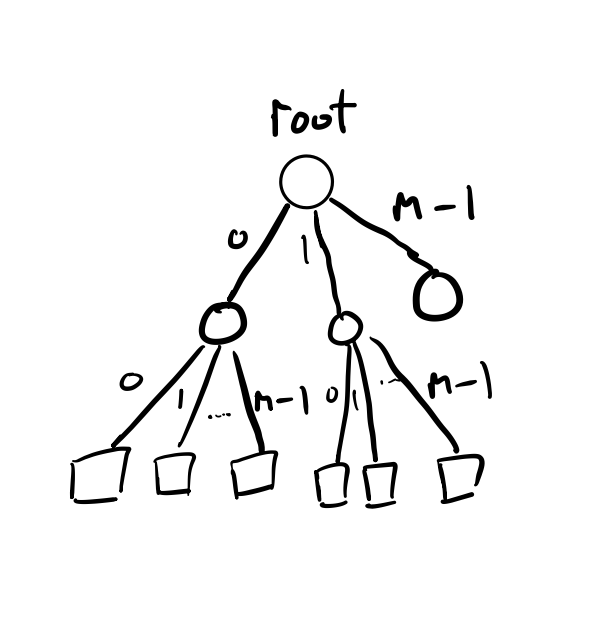
\includegraphics[scale=0.8]{Images/fig-lec1-mary.png}
    \caption{$m$-ary tree $T$}
    \label{lec1-mary}
\end{figure}


This is the mathematical object we work with. How does it do computation? In the way you expect; start at the root and follow the edges based on the labels. Mathematically:

\begin{defbox}{: Deterministic query computation}{}
    Let $T$ be a DDT and $x \in D$. We define $T(x) \in \Gamma$ by the following procedure:
    \begin{enumerate}
        \item Set $v_{\text{current}}$ to be the root vertex.
        \item Repeat the following until the label of a leaf is output:
        \begin{enumerate}[(i)]
            \item If $v_{\text{current}}$ is a leaf, then output its label.
            \item Otherwise, let $i \in [n]$ be the label of $v_{\text{current}}$, and let $v$ be the child of $v_{\text{current}}$ such that the edge $(v, v_{\text{current}})$ is labelled by $x_i$. Set $v_{\text{current}} = v$. 
        \end{enumerate}
    \end{enumerate}
    We say that $T$ computes $f$ if and only if $\forall x \in D, T(x) = f(x)$. 
\end{defbox}
Note: the $\forall$ in the above definition is very important! We are working in the ``worst case''. It has to work for all possible inputs. 

Let's work through the above example with $f(x) = (x_1 \land x_2) \lor (\lnot x_1 \land x_3)$. 

\begin{figure}[htbp!]
    \centering
    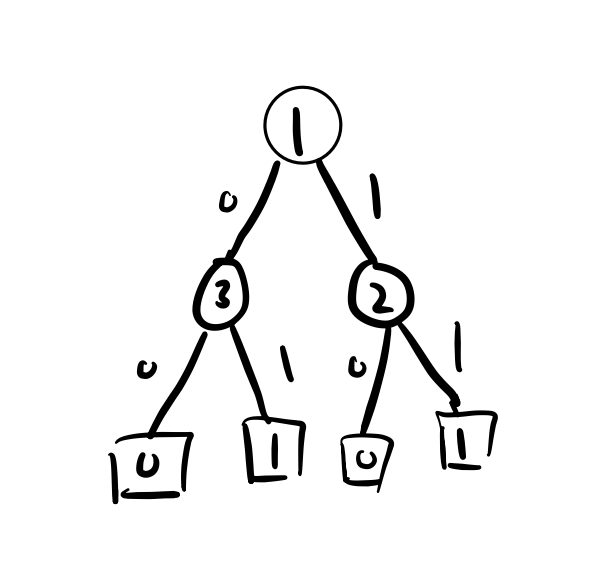
\includegraphics[scale=0.8]{Images/fig-lec1-dtree.png}
    \caption{Minimal depth decision tree that computes $f$}
    \label{lec1-dtree}
\end{figure}

\begin{defbox}{: Deterministic query complexity}{}
    Given a DDT $T$, its depth, denote $\text{depth}(T)$ as the maximum length of a root-to-leaf path. Then:
    \begin{equation}
        D(f) \coloneqq \min_{\text{DDT $T$ computing $f$}}\text{depth}(T)
    \end{equation}
    
\end{defbox}

\begin{defbox}{: Randomized decision tree/query algorithm}{}
    A randomized decision tree (RDT) is a probability distribution over DDTs $\tau = \set{(p_1, T_1), \ldots (p_n, T_k)}$ with $p_i \in [0, 1]$ wiht $\sum_i p_i = 1$. 
\end{defbox}

\begin{defbox}{: Randomized query computation}
    Given $x \in D$ and an RDT $\mathcal{T}$, with $\tau(x)$ for the random variable on $\Gamma$ defined by $\forall i \in \Gamma$ $\text{Pr}[\tau(x) = i] = \text{Pr}[T(x) = i \vert T \leftarrow \tau] = \sum_{j \in [k, T_j(x) = i]}p_j$. Let $\e \in (0, 1/2)$. We say that $\tau$ computes $f$ with bounded error $\e$ if the following holds:
    \begin{equation}
        \forall x \in D, \text{Pr}[\tau(x) = f(x)] \geq 1 - \e = \sum_{j \in [k], T_j(x) = f(x)}p_j
    \end{equation}
\end{defbox}

\begin{defbox}{: Randomixed query complexity}
    Given a RDT $\tau$, its depth $\text{depth}(\tau) = \max_{j \in [k], p_j > 0} (\text{depth}(T_j))$. Then, let $\e \in (0, 1/2)$. Then:
    \begin{equation}
        R_{\e}(f) = \min_{\text{$\tau$ computes $f$ with bounded error $\e$}} \text{depth}(\tau)
    \end{equation}
    It is standard to write $R(f) = R_{1/3}(f)$. 
\end{defbox}